\documentclass[12pt]{article}

\usepackage{amsmath}
\usepackage{unicode-math}
\usepackage{xltxtra}
\usepackage{xgreek}

\setmainfont{Liberation Serif}

\usepackage{tabularx}

\pagestyle{empty}

\usepackage{geometry}
 \geometry{a4paper, total={190mm,275mm}, left=10mm, top=10mm}

 \usepackage{graphicx}
 \graphicspath{ {images/} }

 \usepackage{wrapfig}
\usepackage{lipsum}%% a garbage package you don't need except to create examples.

\begin{document}
  \part*{\centering{Πανελλήνιες Φυσική Γ Λυκείου 2017}}

  \section*{Θέμα Β}
  \begin{enumerate}
    \item [B1-(ii)]

    \begin{figure}[h]
      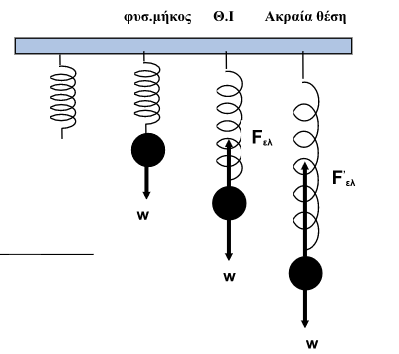
\includegraphics[width=0.4\textwidth]{ΦυσικήΒ1.png}
      \centering
    \end{figure}

    $m$, αατ:

    \begin{gather*}
    (ΘΙ) ΣF=0 \implies \\ F_{ελ}-mg=0 \implies \\ kΔl=mg \implies \\ Δl=\frac{mg}{k}
    \end{gather*}
    Επειδή στη ΘΦΜ $v=0$, άρα $Δl=A$



    $$U_{ελ_{max}}= U_{ελ(Γ')}=\frac{1}{2}k\left(2A\right)^2=\frac{1}{2}4A^2=2k\frac{m^2g^2}{k^2}=\frac{2m^2g^2}{k^2}$$

    άρα σωστό το (ii)

    \item [B2-(iii)]

    Από εξίσωση Bernoulli: $Β\to Γ$
    \begin{figure}[h]
      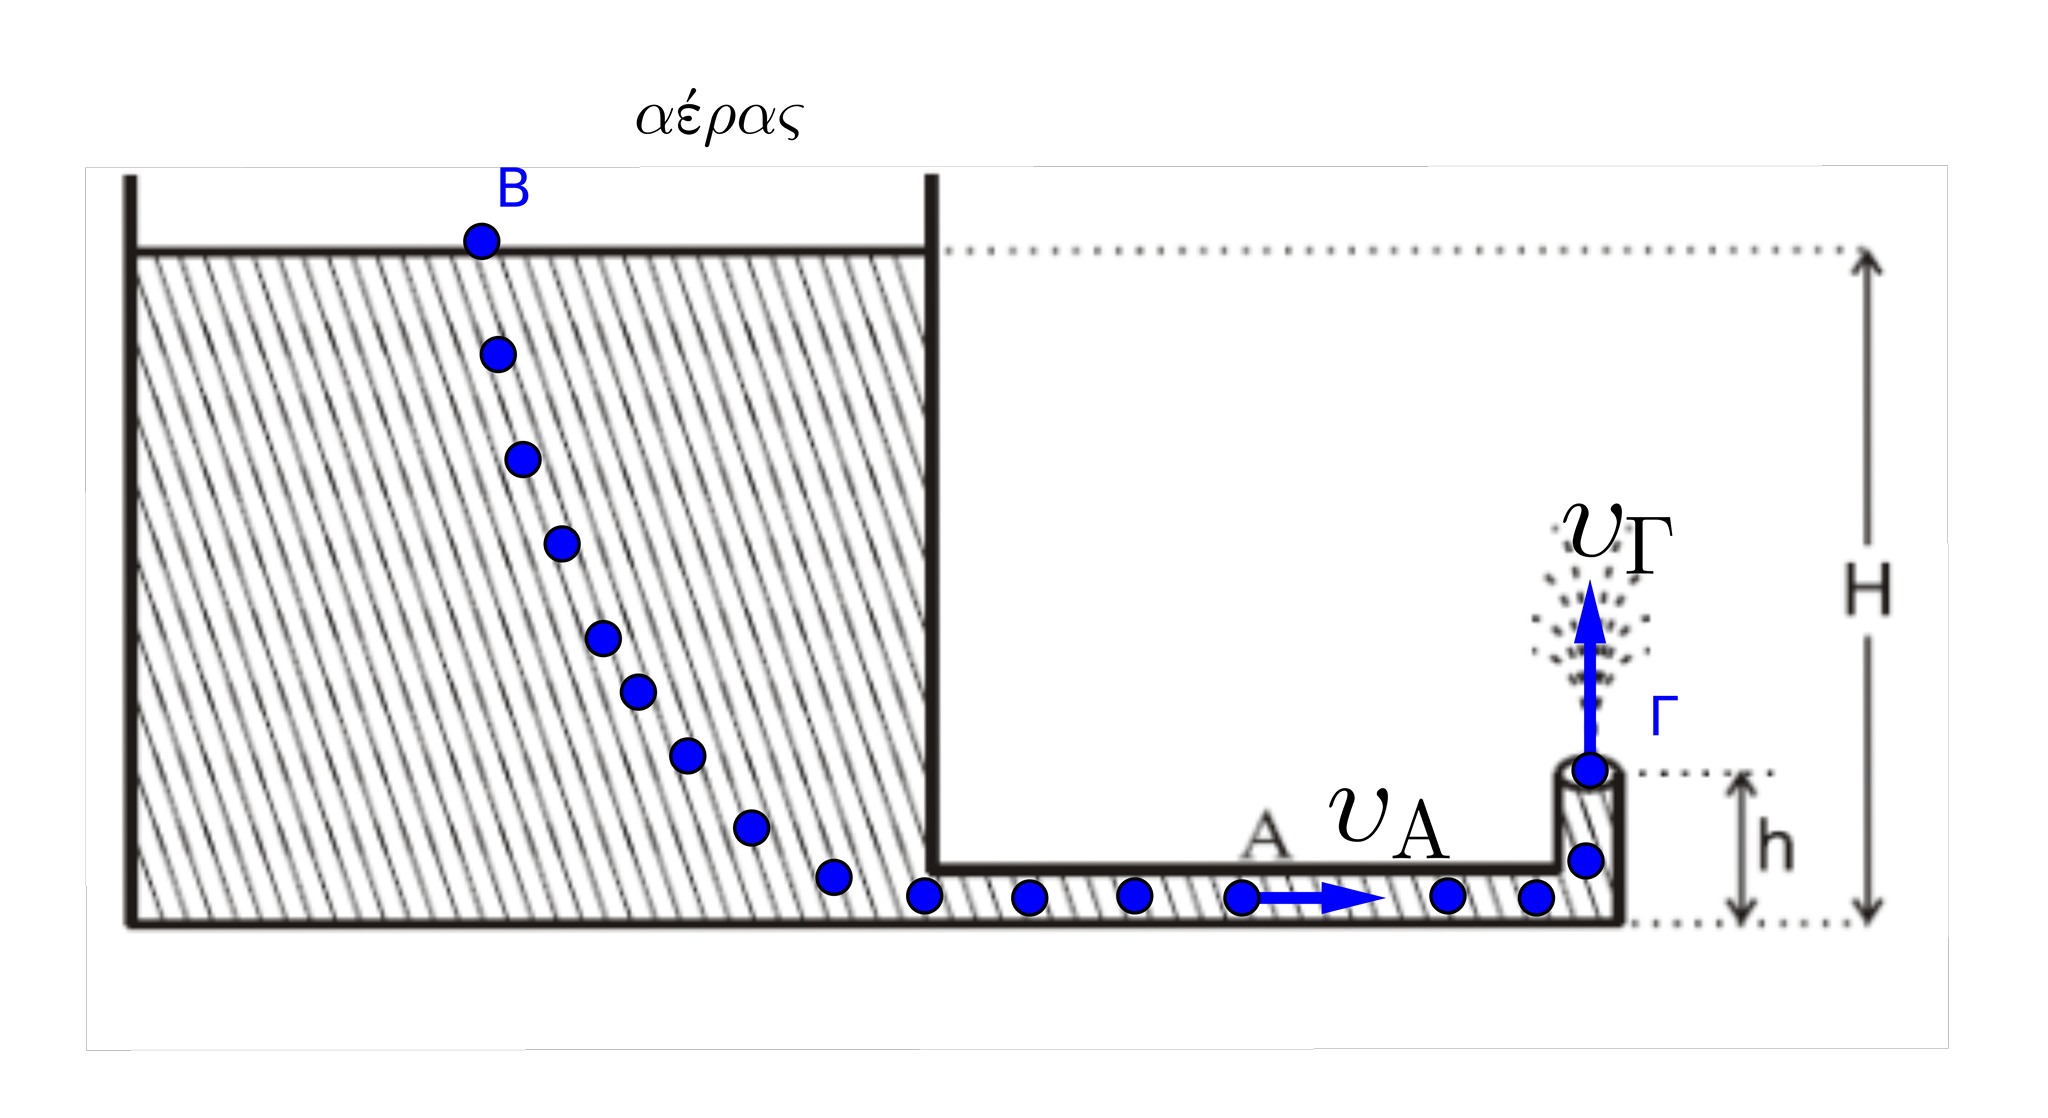
\includegraphics[width=0.5\textwidth]{ΦυσικήΒ2.png}
      \centering
    \end{figure}

    \begin{gather*}
      P_B + \frac{1}{2}ρv_Β^2+ρgH=P_Α+\frac{1}{2}ρv_Α^2+0=
      P_Γ+\frac{1}{2}ρv_Γ^2+ρgh\overset{P_Β=P_Γ=P_{at}}{\underset{v_Β=0}{\implies}}\\
      ρg5h=\frac{1}{2}ρv_Γ^2+ρgh\implies v_Γ^2=8gh\implies v_Γ=2\sqrt{2gh}
    \end{gather*}

    Σύμφωνα με την εξίσωση συνέχειας, η παροχή είναι ίδια για όλα τα σημεία του σωλήνα.
    Άρα η παροχή στα σημεία Α και Γ είναι
    $$Π_Α = Π_Β \implies A_A υ_Α = Α_Γ υ_Γ \implies υ_Α = υ_Γ = 2 \sqrt{2gh}$$
    άρα σωστό το (iii)

    \item [B3-(ii)]
    Ο παρατηρητής $Β$ πλησιάζει την πηγή $Α$ και η πηγή απομακρύνεται από τον παρατηρητή $Β$ άρα θα ισχύει

    \begin{figure}[h]
      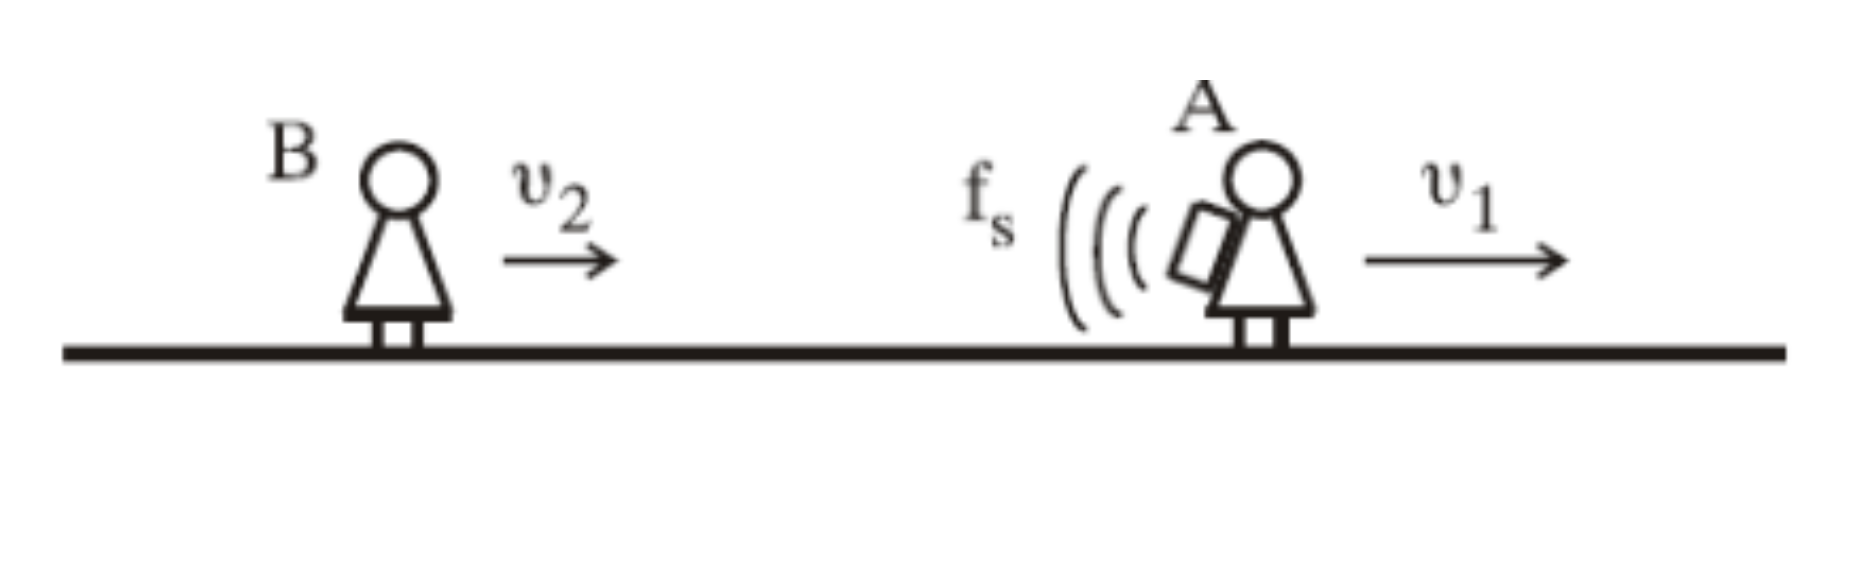
\includegraphics[width=0.4\textwidth]{ΦυσικήΒ3.png}
      \centering
    \end{figure}

    $$f_Β=\dfrac{v_{ηχ}+v_2}{v_{ηχ}+v_1}f_s=\dfrac{v_{ηχ}+\dfrac{v_{ηχ}}{10}}{v_{ηχ}+\dfrac{v_{ηχ}}{5}}f_s=\dfrac{\dfrac{11v_{ηχ}}{10}}{\dfrac{6v_{ηχ}}{10}}f_s=\dfrac{11\cdot5}{10\cdot6}f_s=\dfrac{11}{12}f_s $$

    άρα σωστό το (ii)
  \end{enumerate}

  \section*{Θέμα Γ}
  \begin{enumerate}
    \item [Γ1.]

    \begin{figure}[h]
      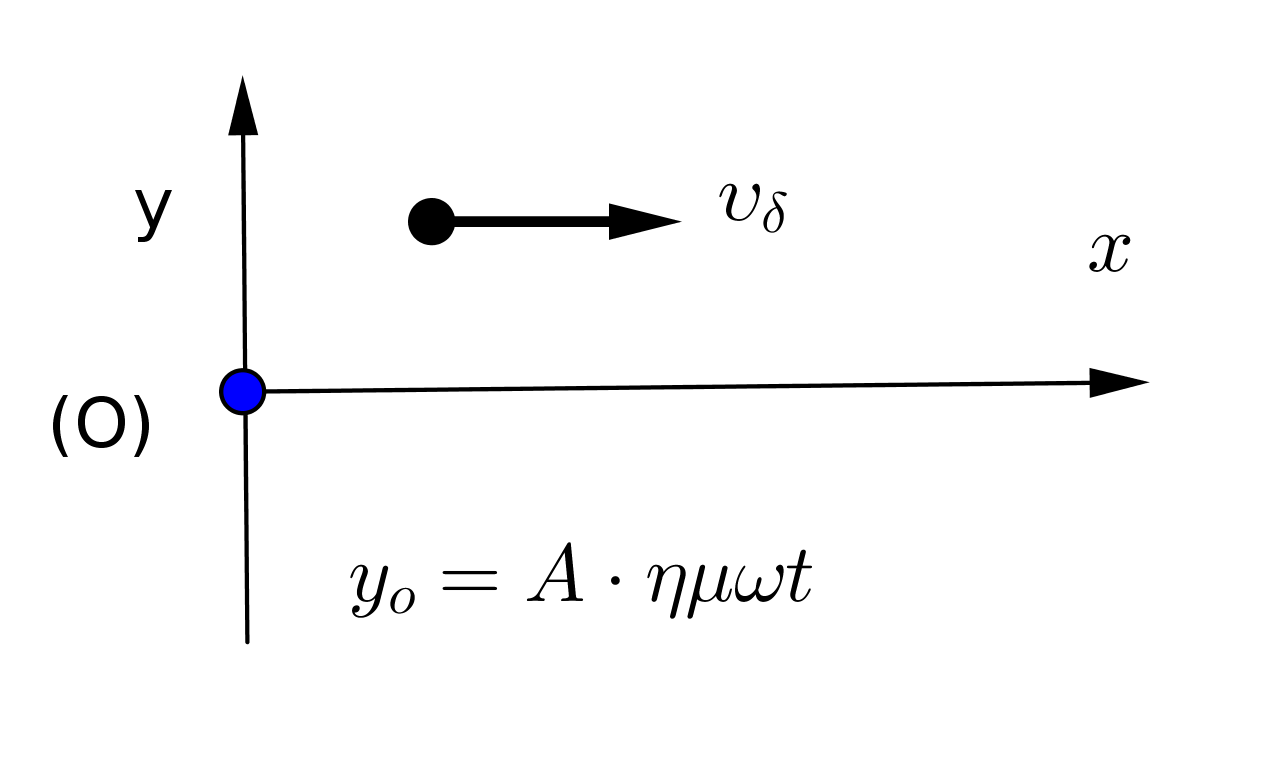
\includegraphics[width=0.4\textwidth]{ΦυσικήΓ1.png}
      \centering
    \end{figure}

      \begin{gather*}
        -A \to +A: Δt=\frac{T}{2}=0,4s\implies T=0,8s
      \end{gather*}
      σε $Δt$ η διαταραχή διαδόθηκε σε απόσταση $Δx=4cm=0,04m$.

      $$v_δ=\frac{Δx}{Δt}=\frac{0,04}{0,4}=0,1m/s$$

      $$v_δ=\frac{λ}{T}\implies λ=0,08m$$

      Το $Δm$ εκτελεί α.α.τ.:

      $$D=Δm\cdot ω^2=Δm\frac{4\pi^2}{T^2}=10^{-6}\frac{4\pi^2}{0,64}=\frac{\pi^2}{16}10^{-4}\frac{N}{m}$$

      $$E_T=\frac{1}{2}D\cdot A^2\implies 5\pi^2 10^{-7}=\frac{1}{2}\cdot\frac{\pi^2}{16}10^{-4}A^2\implies A^2=0,16\implies A=0,4m \text{ (πλάτος)}$$

    \item [Γ2.]

    Η εξίσωση του κύματος είναι:

    $$y_{(x,t)}=Aημ\left(\frac{2\pi t}{T}-\frac{2\pi x}{λ}\right)=0,4ημ\left(\frac{5\pi t}{2}-25\pi x \right) \text{ (SI)}$$

    Στιγμιότυπο την $t_1=1,4s$:

    \begin{gather*}
      \begin{matrix}
        \text{Την }t_1 \text{ η διαταραχή} \\ \text{έφτασε στη θέση }
      \end{matrix}
       \left\{ \begin{matrix}
        x_1=v_δ t_1=0,1\cdot 1,4=0,14m, N_1=\frac{x_1}{λ}=\frac{0,14}{0,08}=\frac{14}{8}=\frac{7}{4} \text{ μήκη κύματος} \\
        \text{ ή } \\
        φ_{t_1}=0\implies \frac{5\pi \cdot 1,4}{2}-25\pi x_1=0\implies x_1=0,14m
      \end{matrix} \right.
    \end{gather*}

        \begin{figure}[h]
          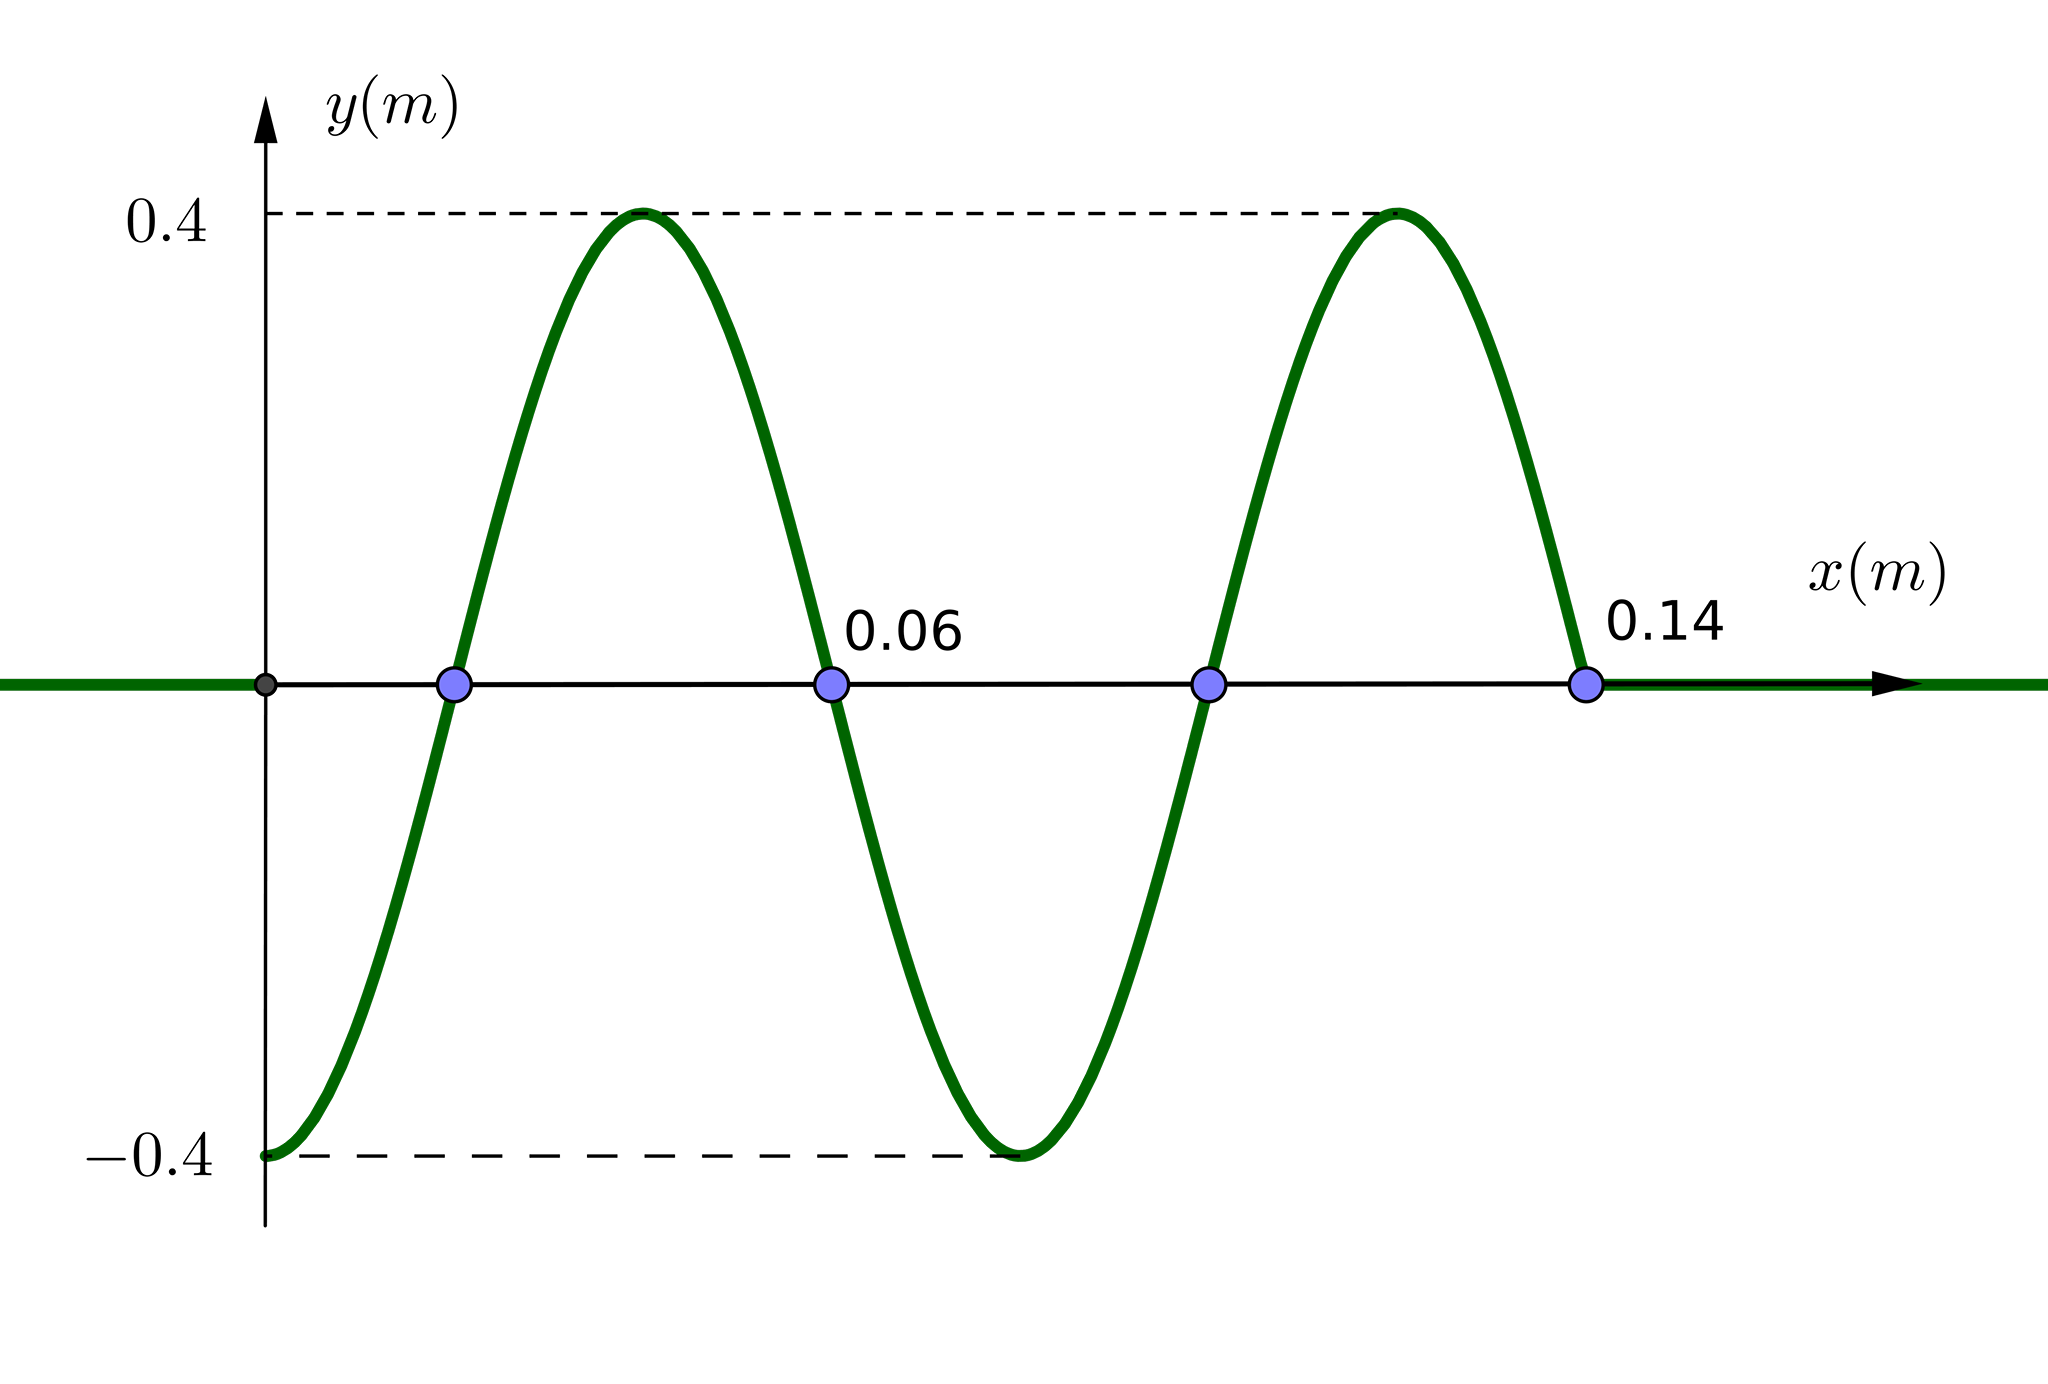
\includegraphics[width=0.4\textwidth]{ΦυσικήΓ2.png}
          \centering
        \end{figure}

    $$y_{t_1}=\begin{cases}
      0,4ημ\left(3,5\pi-25\pi x \right), & 0\le x\le 0,14m \\
      0, & 0,14m < x
    \end{cases}$$

    $$x=0,y_{0}=0,4ημ3,5\pi=-0,4m$$

    \item [Γ3.]
      $ΑΔΕ_{ταλ}$ για $Δm$

      Για $$y=0,2m=\frac{A}{2}$$

      \begin{gather*}
        E_T=K+U\implies E_T=K+\frac{1}{2}Dy^2 \overset{y=\frac{A}{2}}{\implies} E_T=K+\frac{1}{2}D\frac{A^2}{4}\implies \\ E_T=K+\frac{1}{4}E_T\implies K=\frac{3}{4}E_T=\frac{3}{4}5\pi^2 10^{-7}=\frac{3\pi^2}{8}10^{-6} J
      \end{gather*}

      ή

      $$y=Aημφ=\frac{A}{2}\implies ημφ=\frac{1}{2}\implies φ=\begin{cases}2k\pi+\frac{\pi}{6}, & k=0,1,2,... (1) \\ 2k\pi + \frac{5\pi}{6}, & k = 0,1,2,... (2)\end{cases}$$

      $$v=ωAσυνφ=\begin{cases}=ωAσυν\left(2k\pi+\frac{\pi}{6}\right)=\frac{ωA\sqrt{3}}{2} \\ ωAσυν\left(2k\pi+\frac{5\pi}{6}\right)=-\frac{ωA\sqrt{3}}{2}\end{cases}$$

      $$K=\frac{1}{2}Δm\cdot v^2=\frac{1}{2}Δm\left(\pm \frac{ωA\sqrt{3}}{2} \right)^2=\frac{1}{2}Δm\cdot \frac{ω^2A^2 3}{4}=\frac{3}{4}\cdot\frac{1}{2}D\cdot A^2=\frac{3}{4}E_T$$

      \item [Γ4.]

      \begin{figure}[h]
        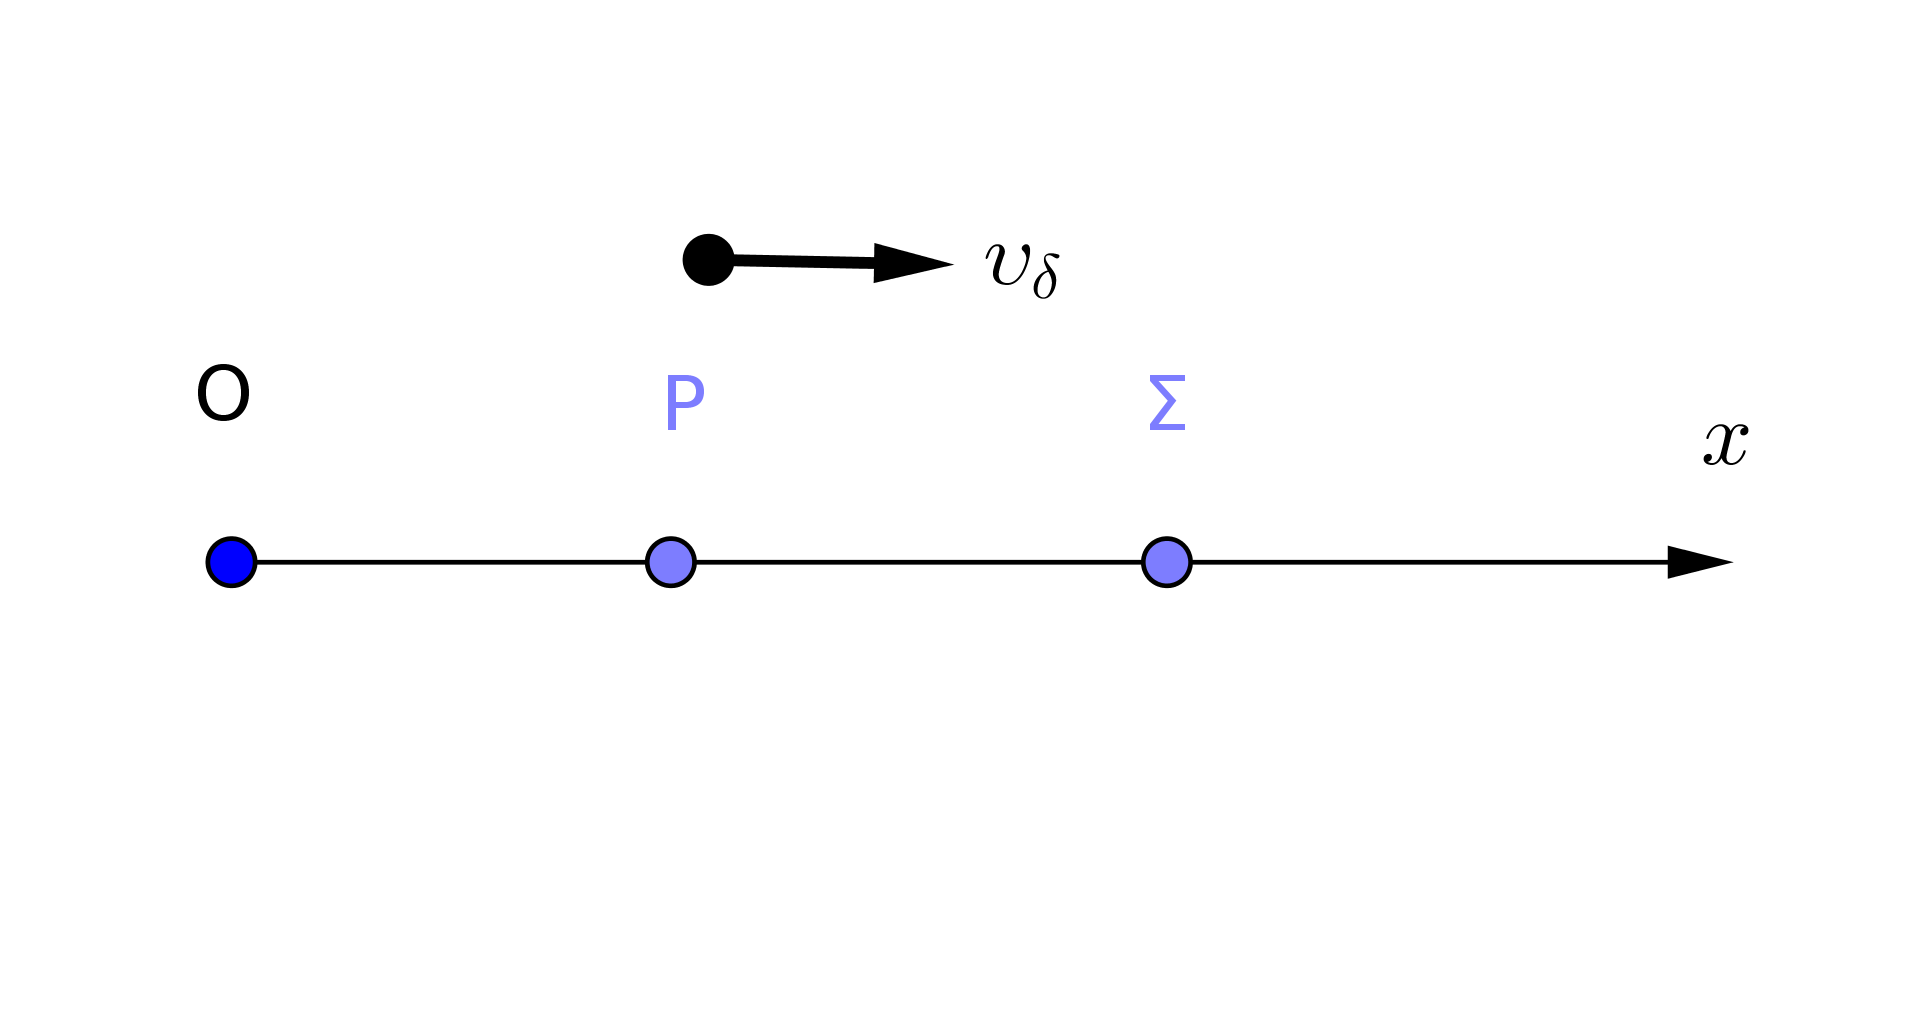
\includegraphics[width=0.5\textwidth]{ΦυσικήΓ4.png}
        \centering
      \end{figure}

      $$φ_Ρ-φ_Σ=\frac{3\pi}{2}rad,(φ_Ρ>φ_Σ)$$

      $$\left. \begin{matrix}y_Ρ=0,4m=A \\ y_Ρ=Aημφ_Ρ\end{matrix} \right\} ημφ_Ρ=1\implies φ_Ρ=2k\pi+\frac{\pi}{2},k=0,1,2,\ldots$$

      $$2k\pi+\frac{\pi}{2}-φ_Σ=\frac{3\pi}{2}\implies φ_Σ=2k\pi-\pi$$
      Άρα

      $$v_Σ=\frac{5\pi}{2}\cdot 0,4\cdot συν\left(2k\pi-\pi\right)\implies v_Σ=-\pi \frac{m}{s}$$

      ή

      \begin{gather*}
        φ_Ρ-φ_Σ=\frac{3\pi}{2}\implies \\
        \left. \begin{matrix}\frac{5\pi t}{2}-25\pi x_Ρ-\left(\frac{5\pi t}{2}-25\pi x_Σ\right)=\frac{3\pi}{2}\implies x_Σ-x_Ρ=\frac{3}{50} \\ \frac{2\pi t}{T}-\frac{2\pi x_Ρ}{λ}-\left(\frac{2\pi t}{T}-\frac{2\pi x_Σ}{λ}\right)=\frac{3\pi}{2}\implies x_Σ-x_Ρ=\frac{3λ}{4}\end{matrix} \right\}\implies \frac{3λ}{4}=\frac{3}{50}\implies λ=0,08=\frac{4}{50}m
      \end{gather*}


      \begin{figure}[h]
        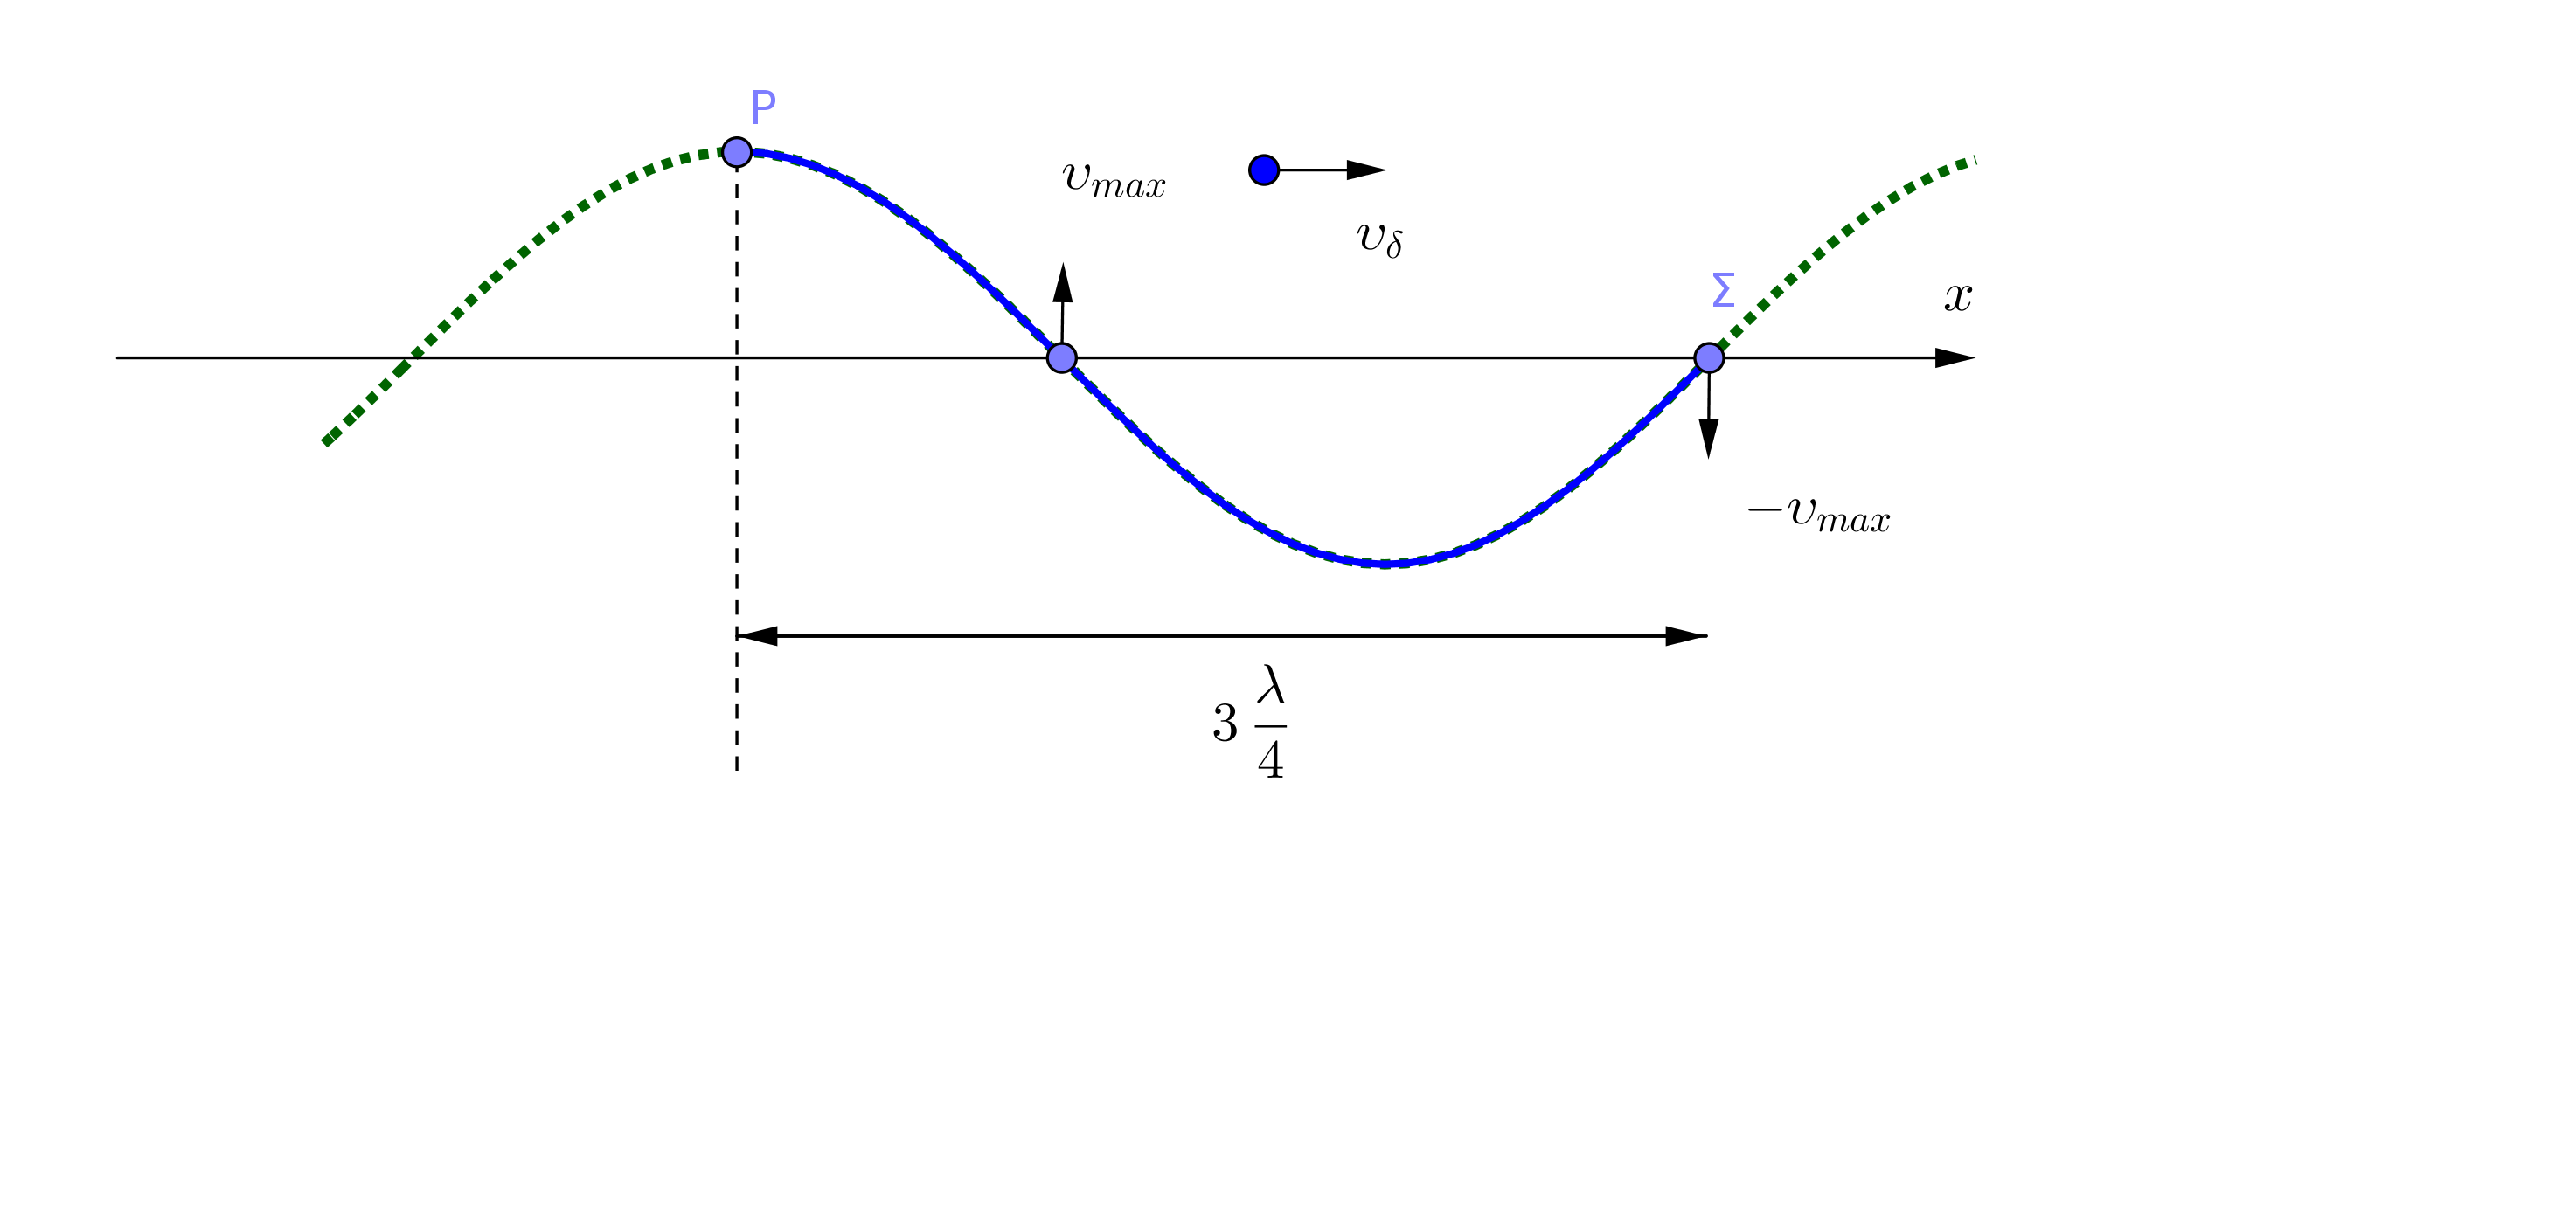
\includegraphics[width=0.8\textwidth]{ΦυσικήΓ4_2.png}
        \centering
      \end{figure}

      όταν $y_Ρ=A$, $$v_Σ=-ωA=-\pi \frac{m}{s}$$
  \end{enumerate}

  \section*{Θέμα Δ}

  \begin{enumerate}
    \item [Δ1.]

    \begin{gather*}
      \left. \begin{matrix}ΣF=m\cdot a_{cm}\implies W-T_1=m\cdot a_{cm} \\ Σ\uptau=Iα_{γων}\implies T_1\cdot R=\frac{1}{2}mR^2\cdot α_{γων}\end{matrix} \right\} \\
      T_1=\frac{m\cdot a_{cm}}{2},W=\frac{3m\cdot a_{cm}}{2}
    \end{gather*}

    \begin{figure}[h]
      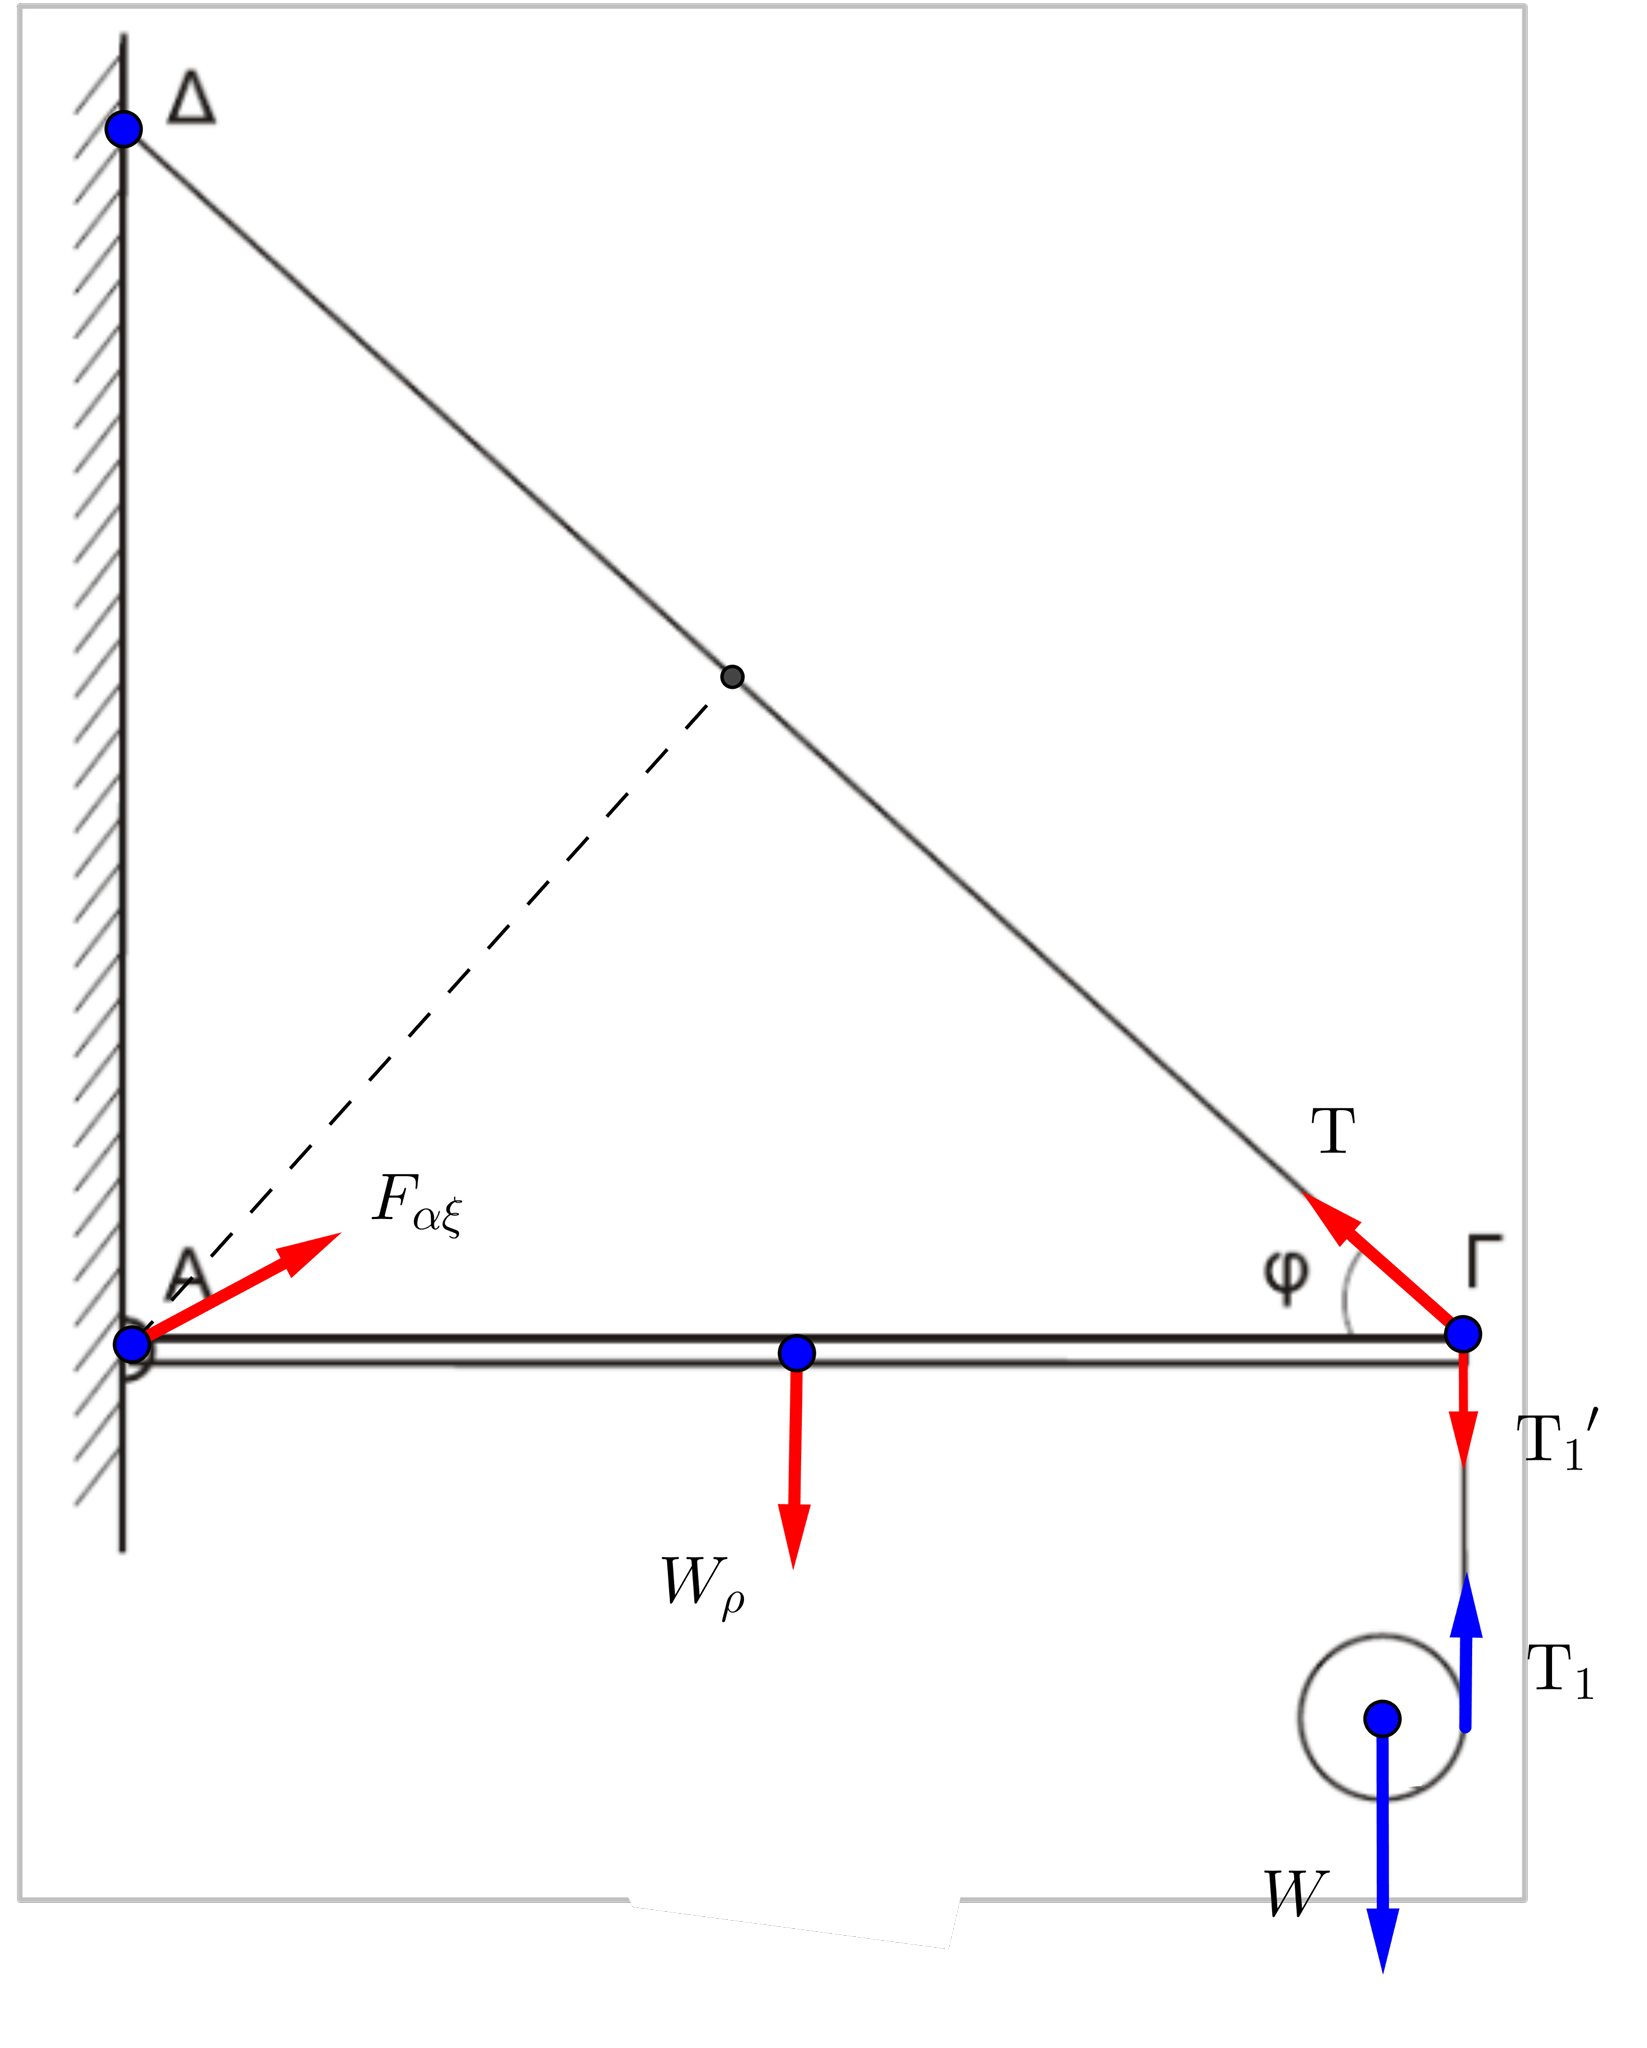
\includegraphics[width=0.3\textwidth]{ΦυσικήΔ1.png}
      \centering
    \end{figure}

    $$0=v_Γ=v_Z=v_{cm}-v_{γρ_Ζ}\implies v_{cm}=ωR\implies a_{cm}=a_γ R\implies a_{cm}=\frac{2}{3}g=\frac{20}{3}\frac{m}{s}$$

    \item [Δ2.]

    $$T'_1=T_1=\frac{2\cdot 20}{2\cdot 3}=\frac{20}{3}N$$
  
    3ος Νόμος του Νεύτωνα και νήμα αβαρές μη εκτατό

    Για τη ράβδο που ισορροπεί:

    $$Σ_{τ_{(Α)}}=0\implies w_ρ\cdot\frac{l}{2}+T'_1\cdot l-T\cdot l\cdot ημφ=0\implies T=\frac{100}{3}N$$

    \item [Δ3.]


    \begin{figure}[h]
      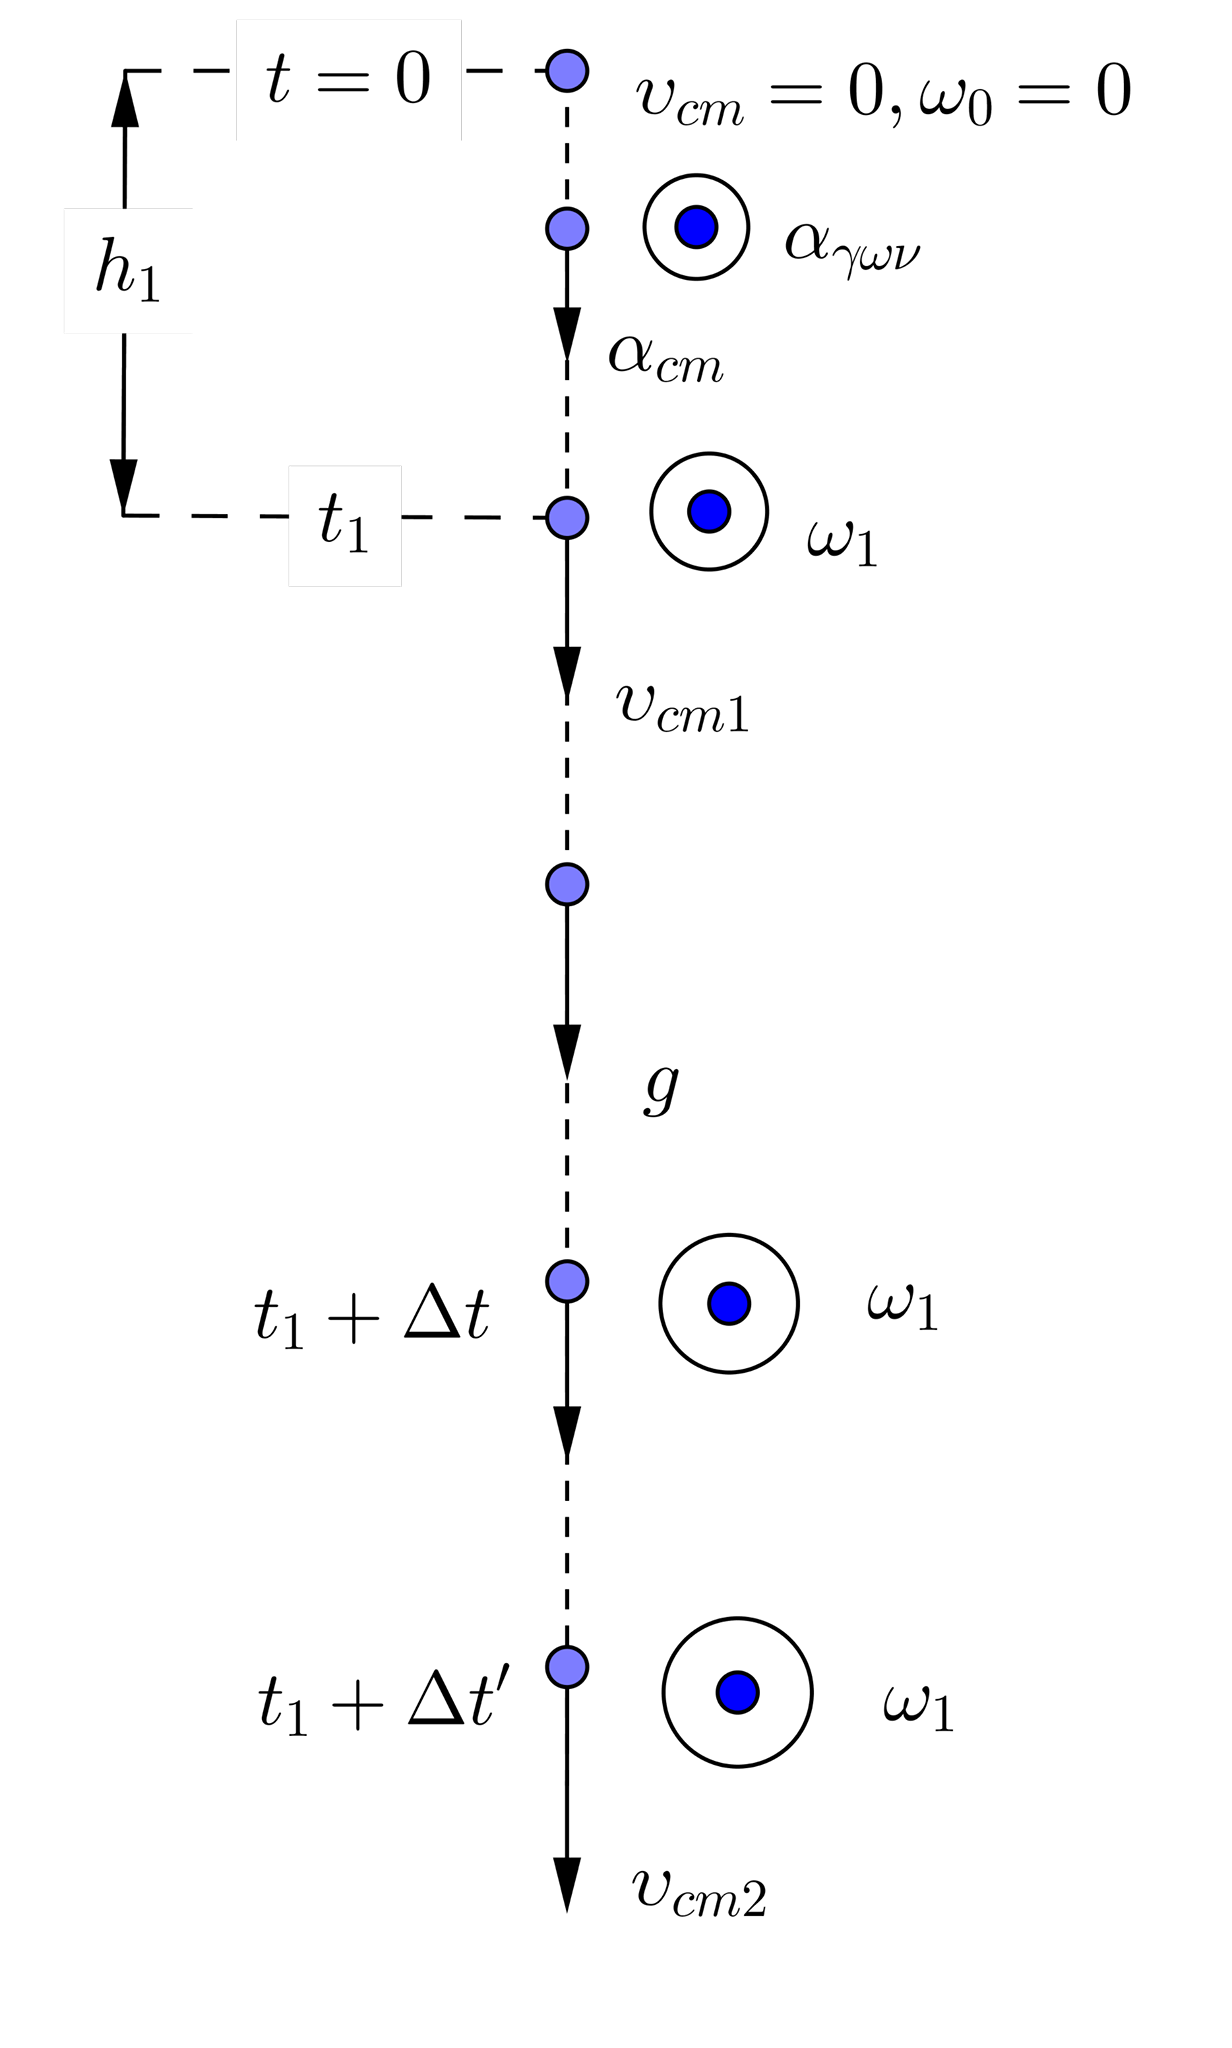
\includegraphics[width=0.3\textwidth]{ΦυσικήΔ3.png}
      \centering
    \end{figure}

    Την $t_1$, $h_1=0,3m$

    $$h_1=\frac{1}{2}a_{cm}t_1^2\implies 0,3=\frac{1}{2}\cdot\frac{20}{3}t_1^2\implies t_1=0,3s$$

    $$a_{γων}=\frac{a_{cm}}{R}=\frac{200}{3}r/s^2$$

    $$w_1=a_{γων}t_1=20r/s$$

    $t \to t_1+Δt$:

    $$\uptau_{w_{cm}}=0=\frac{ΔL}{Δt}\implies L_{t_1}=L_{t_1+Δ_t}$$

    Η μόνη δύναμη που ασκείται στο δίσκο είναι το βάρος $W$.

    Όπου

    $$L_{t_1}=I\cdot ω_1$$

    $$I=\frac{1}{2}mR^2=\frac{1}{2}\cdot 2 \cdot 0,1^2=0,01kg m^2$$

    Άρα

    $$L_{t_1}=0,2kg\frac{m^2}{s}=L_{t_1+Δt}$$

    ή $ΘΜΚΕ_{(0\to h_1)}:$

    \begin{gather*}
      \left. \begin{matrix}\text{μετ: }\frac{1}{2}mv_{cm1}^2-0=W\cdot h_1-T_1\cdot h_1 \\ \text{στρ: } \frac{1}{2}Iω_1^2-0=+(T_1\cdot R)\cdot θ_1 \\ v_{cm1}=ω_1\cdot R \\ x_{cm}=θ\cdot R\implies h_1=θ_1\cdot R \end{matrix} \right\}\implies \\      \frac{1}{2}mv_{cm1}^2+\frac{1}{2}Iω_1^2=mgh_1\implies  \\
      \frac{1}{2}v_{cm1}^2+\frac{1}{4}\cdot v_{cm1}^2=gh_1 \implies v_{cm1}^2=\frac{4gh_1}{3}\implies v_{cm1}=2m/s \implies ω_1=20r/s \implies \\
       L_{t_1}=Iω_1=0,2kg \frac{m^2}{s}\implies L_{t_1}=0,2 kg \frac{m^2}{s}
    \end{gather*}

    Η δύναμη $T_1$ δε μετατοπίζει το σημείο εφαρμογής της, αφού κάθε στιγμή ασκείται σε διαφορετικό σημείο του δίσκου, λειτουργεί δηλαδή όπως η στατική τριβή στη Κ.Χ.Ο. Επομένως η μηχανική ενέργεια του δίσκου διατηρείται.

    $ΑΔΜΕ_{(0,h_1)}:$

    \begin{gather*}
      K_{(0)}+U_{(0)}=K_{(t_1)}+U_{(t_1)} \\      0+mgh_1=\left( \frac{1}{2}mv_{cm1}^2+\frac{1}{2}Iω_1^2\right) + 0 \\
      mgh_1=\frac{1}{2}mω_1^2R^2+\frac{1}{2}Iω_1^2 \\
      mgh_1=Iω_1^2+\frac{1}{2}Iω_1^2=3\cdot\frac{1}{2}Iω_1^2 \\
      \left. \begin{matrix} \left.
        \begin{matrix}K_{στρ}=\frac{1}{2}Iω_1^2 \\ L=Iω_1
        \end{matrix}
        \right\} K_{στρ}=\frac{L^2}{2I} \\
        mgh_1=3K_{(στρ)}
      \end{matrix}
      \right\}
      \implies mgh_1=\frac{3L^2}{2I} \\
      9\cdot 10\cdot 0,3=\frac{3L_{t_1}^2}{2\cdot 0,01}
      \implies L_{t_1}=0,2kg \frac{m^2}{s} \\
    \end{gather*}

    \item [Δ4.]
    $t_2=t_1+Δt'$:

    \begin{gather*}
      \frac{K_{στρ(t_2)}}{K_{μετ(t_2)}}=\frac{\frac{1}{2}Iω_2^2}{\frac{1}{2}mv_{cm_2}^2}
    \end{gather*}

    $t_1=t_2$:

    \begin{gather*}
      Σ\uptau_{cm}=0\implies ω_2=ω_1=20r/s \\
      ΣF=m\cdot a_{cm}\implies W=m\cdot a_{cm}\implies a_{cm}=g=10 m/s^2 \\
      v_{cm_2}=v_{cm_1}+g\cdot Δt'=2+10\cdot 0,1=3m/s
    \end{gather*}

    \begin{gather*}
      \frac{K_{περ}}{K_{μετ}}=\frac{\frac{1}{2}Iω^2}{\frac{1}{2}mv^2}=\frac{\frac{1}{2}mR^2ω_2^2}{mv_2^2}=\frac{2}{9} \\
      \frac{K_{περ}}{K_{μετ}}=\frac{2}{9}
    \end{gather*}

  \end{enumerate}

\end{document}
